\documentclass[11pt,british,a4paper]{report}
%\pdfobjcompresslevel=0
%\usepackage{pythontex}
\usepackage[usenames,dvipsnames]{xcolor}
\usepackage[includeheadfoot,margin=0.8 in]{geometry}
\usepackage{siunitx,physics,cancel,upgreek,varioref,listings,booktabs,pdfpages,ifthen,polynom,todonotes}
%\usepackage{minted}
\usepackage[backend=biber]{biblatex}
\DefineBibliographyStrings{english}{%
      bibliography = {References},
}
\addbibresource{sources.bib}
\usepackage{mathtools,upgreek,bigints}
\usepackage{babel}
\usepackage{graphicx}
\graphicspath{{./}{./e/}}
\usepackage{float}
\usepackage{amsmath}
\usepackage{amssymb,epstopdf}
\usepackage{enumitem}
\usepackage[T1]{fontenc}
%\usepackage{fouriernc}
% \usepackage[T1]{fontenc}
\usepackage{mathpazo}
% \usepackage{inconsolata}
%\usepackage{eulervm}
%\usepackage{cmbright}
%\usepackage{fontspec}
%\usepackage{unicode-math}
%\setmainfont{Tex Gyre Pagella}
%\setmathfont{Tex Gyre Pagella Math}
%\setmonofont{Tex Gyre Cursor}
%\renewcommand*\ttdefault{txtt}
\usepackage[scaled]{beramono}
\usepackage{fancyhdr}
\usepackage[utf8]{inputenc}
\usepackage{textcomp}
\usepackage{lastpage}
\usepackage{microtype}
\usepackage[font=normalsize]{subcaption}
\usepackage{luacode}
\usepackage[linktoc=all, bookmarks=true, pdfauthor={Anders Johansson},pdftitle={FYS-MEK-project}]{hyperref}
\usepackage{tikz,pgfplots,pgfplotstable}
\usepgfplotslibrary{colorbrewer}
\usepgfplotslibrary{external}
\tikzset{external/system call={lualatex \tikzexternalcheckshellescape -halt-on-error -interaction=batchmode -jobname "\image" "\texsource"}}
\tikzexternalize[prefix=tmp/, mode=list and make]
\pgfplotsset{cycle list/Dark2}
\pgfplotsset{compat=1.8}
\renewcommand{\CancelColor}{\color{red}}
\let\oldexp=\exp
\renewcommand{\exp}[1]{\mathrm{e}^{#1}}
\renewcommand{\Re}[1]{\mathfrak{Re}\ifthenelse{\equal{#1}{}}{}{\left(#1\right)}}
\renewcommand{\Im}[1]{\mathfrak{Im}\ifthenelse{\equal{#1}{}}{}{\left(#1\right)}}
\renewcommand{\i}{\mathrm{i}}
\newcommand{\tittel}[1]{\title{#1 \vspace{-7ex}}\author{}\date{}\maketitle\thispagestyle{fancy}\pagestyle{fancy}\setcounter{page}{1}}

% \newcommand{\deloppg}[2][]{\subsection*{#2) #1}\addcontentsline{toc}{subsection}{#2)}\refstepcounter{subsection}\label{#2}}
% \newcommand{\oppg}[1]{\section*{Oppgave #1}\addcontentsline{toc}{section}{Oppgave #1}\refstepcounter{section}\label{oppg#1}}

\labelformat{section}{#1}
\labelformat{subsection}{exercise~#1}
\labelformat{subsubsection}{paragraph~#1}
\labelformat{equation}{equation~(#1)}
\labelformat{figure}{figure~#1}
\labelformat{table}{table~#1}


%\setcounter{secnumdepth}{4}
\renewcommand{\thesection}{Part \arabic{section}}
\renewcommand{\thesubsection}{\arabic{section}\alph{subsection})}
\renewcommand{\thesubsubsection}{\arabic{section}\alph{subsection}\roman{subsubsection})}
\setlength{\parindent}{0cm}
\setlength{\parskip}{1em}

\definecolor{bluekeywords}{rgb}{0.13,0.13,1}
\definecolor{greencomments}{rgb}{0,0.5,0}
\definecolor{redstrings}{rgb}{0.9,0,0}
\lstset{rangeprefix=\#!,
    rangesuffix=!\#,
    includerangemarker=false}
\lstset{showstringspaces=false,
    basicstyle=\small\ttfamily,
    keywordstyle=\color{bluekeywords},
    commentstyle=\color{greencomments},
    numberstyle=\color{bluekeywords},
    stringstyle=\color{redstrings},
    breaklines=true,
    texcl=true,
    language=Python
}
\colorlet{DarkGrey}{white!20!black}
\newcommand{\eqtag}[1]{\refstepcounter{equation}\tag{\theequation}\label{#1}}
\hypersetup{hidelinks=True}

\sisetup{detect-all}
\sisetup{exponent-product = \cdot, output-product = \cdot,per-mode=symbol}
% \sisetup{output-decimal-marker={,}}
\sisetup{round-mode = off, round-precision=3}
\sisetup{number-unit-product = \ }

\allowdisplaybreaks[4]
\fancyhf{}

% \rhead{MD-Project}
\rfoot{Page~\thepage{} of~\pageref{LastPage}}
% \lhead{FYS-MEK1110}
\renewcommand{\headrulewidth}{0pt}
\renewcommand{\footrulewidth}{\headrulewidth}

%\definecolor{gronn}{rgb}{0.29, 0.33, 0.13}
\definecolor{gronn}{rgb}{0, 0.5, 0}

\newcommand{\husk}[2]{\tikz[baseline,remember picture,inner sep=0pt,outer sep=0pt]{\node[anchor=base] (#1) {\(#2\)};}}
\newcommand{\artanh}[1]{\operatorname{artanh}{\qty(#1)}}
\newcommand{\matrise}[1]{\begin{pmatrix}#1\end{pmatrix}}

\newread\infile

%start
\begin{document}
%\maketitle

\begin{titlepage}
%\includegraphics[width=\textwidth]{fysisk.pdf}
\vspace*{\fill}
\begin{center}
\textsf{
    \Huge \textbf{Molecular Dynamics Project}\\\vspace{0.5cm}
    \Large \textbf{FYS-MEK1110 --- Mechanics}\\
    \vspace{8cm}
    \begin{tabular}{lr}
        Deadline: & 30th February 2019\\
        Last updated: & \today
    \end{tabular}\\
}
\vspace{1.5cm}

\includegraphics{uio.pdf}\\
\vspace*{\fill}
\end{center}
\end{titlepage}
\null
\pagestyle{empty}
\newpage

\pagestyle{fancy}
\setcounter{page}{1}
\setcounter{section}{-1}

\section{\underline{Practical information}}
This project is meant as a more challenging alternative to the first three mandatory assignments for those who feel that they already have a good grasp of high school physics, basic scientific programming and the Forward Euler method. The workload is (hopefully) approximately equal to the combined workload of the first three assignments.

A special weekly group session will focus on this project, where you can discuss with fellow students and get help from teaching assistants. Additionally, you are encouraged to use the Piazza platform for asking your own questions and answering the questions of other students.

If you at some point find that this project is too difficult or time-consuming for you, the work you have already done may replace one or two normal assignments depending on how far you have come. Let us know, and we will find a solution.

Since this project dives deeply into one subject, it touches on fewer topics from the syllabus than the ordinary assignments. If you choose to do this project, it is therefore especially important that you also do the weekly exercises and attend normal group sessions.

Python and Matlab are the natural choices of programming language for this project. You are allowed to choose any other language, especially fast languages such as Fortran and C++, but you cannot expect all teaching assistants to know all programming languages.

When writing your programs, you should keep two things in mind:
\begin{itemize}
    \item Reusability: This project contains many exercises, but most of them are variants of or build upon earlier exercises, so you will save a lot of time if your implementation is easy to extend or adapt to a new problem.
    \item Efficiency: The two last parts of the project require larger simulations which will run for hours (or even days) if your program is slow. Try therefore to think of efficiency, and use vectorised operations with Numpy arrays whenever possible. Use your own time wisely as well, e.g.\ by writing answers to the exercises while your programs are running.
\end{itemize}

In the end, we hope that you will enjoy the project and your introduction to the world of molecular dynamics. If you do, make sure to check out the summer scholarships offered in molecular dynamics by the Centre for Computing in Science Education (CCSE).

Good luck!


\clearpage

%  _       _                 _       _         _
% (_)_ __ | |_ _ __ ___   __| |_   _| | _____ (_) ___  _ __
% | | '_ \| __| '__/ _ \ / _` | | | | |/ / __|| |/ _ \| '_ \
% | | | | | |_| | | (_) | (_| | |_| |   <\__ \| | (_) | | | |
% |_|_| |_|\__|_|  \___/ \__,_|\__,_|_|\_\___// |\___/|_| |_|
%                                           |__/
\section{\underline{Introduction}}
In this project, you will learn the basics of a simulation technique called molecular dynamics (MD). Molecular dynamics is a method actively used in research here at the Department of Physics, yet its basic principle can be understood and implemented with the background of a first-year physics student.

Molecular dynamics is based on the assumption that even atoms move according to the laws of Newton, given the correct model for interactions. The goal of this project is to model an argon gas, where the atoms interact according to the famous Lennard-Jones potential,
\begin{equation}
    U(r) = 4\varepsilon\qty(\qty(\frac{\sigma}{r})^{12} - \qty(\frac{\sigma}{r})^6), \label{eq:lj}
\end{equation}
where \(r\) is the distance between two atoms, \(r=\norm{\vec{r}_i-\vec{r}_j}\). \(\sigma\) and \(\varepsilon\) are parameters which determine which chemical compound is modelled. This potential is a good approximation for noble gases.

\subsection{Understanding the potential}\label{subsec:understanding}
\begin{enumerate}[label=\roman*.]
    \item Plot the potential as a function of \(r\) with \(\varepsilon=1\) and \(\sigma=1\).
    \item The behaviour of \(U(r)\) is vastly different for \(r \ll \sigma\) and \(r \gg \sigma\). Which term in the potential,~\vref{eq:lj}, dominates in each case and what is the effect?
    \item Find and characterise the equilibrium points of the potential.
    \item Describe qualitatively the motion of two atoms which start at rest separated by a distance of \(\num{1.5}\sigma\). What if they start with a separation of \(\num{0.95}\sigma\)?  (Hint: use the graph of the potential.)
    \item Describe the shape of the potential close to the stable equilibrium point. Can you think of other force(s) with the same behaviour?
\end{enumerate}

\subsection{Forces and equations of motion}
\begin{enumerate}[label=\roman*.]
    \item Find the force on atom \(i\) at position \(\vec{r}_i\) from atom \(j\) at position \(\vec{r}_j\).
    \item Show that the equation of motion for atom \(i\) is
    \begin{equation}
        \dv[2]{\vec{r}_i}{t} = \frac{24\varepsilon}{m} \sum_{j \neq i} \qty(2\qty(\frac{\sigma}{\norm{\vec{r}_i-\vec{r}_j}})^{12}-\qty(\frac{\sigma}{\norm{\vec{r}_i-\vec{r}_j}})^6)\frac{\vec{r}_i-\vec{r}_j}{\norm{\vec{r}_i-\vec{r}_j}^2}.
    \end{equation}
\end{enumerate}

\subsection{Units}
As you may remember from MAT-INF1100, numerical accuracy is reduced when computing with values which are many orders of magnitude apart. This is often an issue in physics, and molecular dynamics is no exception. For example, the mass of argon is smaller than \(10^{-25}\ \si{\kg}\), while typical length scales are on the order of nanometres, \(10^{-9}\ \si{\m}\).

The remedy is to change units so that most quantities are close to \(1\). From~\vref{eq:lj} it is clear that \(\sigma\) and \(\varepsilon\) are the typical scales for length and energy.

\begin{enumerate}[label=\roman*.]
    \item Introduce the scaled coordinates \(\vec{r}_i\,'=\vec{r}_i/\sigma\) and show that the equation of motion can be rewritten in terms of these coordinates as
    \begin{equation}
        \dv[2]{\vec{r}_i\,'}{{t'}} = 24 \sum_{j \neq i} \qty(2\norm{\vec{r}_i\,'-\vec{r}_j\,'}^{-12}-\norm{\vec{r}_i\,'-\vec{r}_j\,'}^{-6})\frac{\vec{r}_i\,'-\vec{r}_j\,'}{\norm{\vec{r}_i\,'-\vec{r}_j\,'}^2},\label{eq:undim}
    \end{equation}
    where \(t'=t/\tau\) for a suitable choice of \(\tau\).
    \item What is the characteristic time scale \(\tau\), and what is its value for argon, which has \(\sigma=\SI{3.405}{\angstrom}\) (\(\SI{1}{\angstrom}=\SI{1e-10}{\m}\)), \(m = \SI{39.95}{\atomicmassunit}\) (\(\SI{1}{\atomicmassunit} = \SI{1.66e-27}{\kg}\)) and \(\varepsilon=\SI{1.0318e-2}{\eV}\) (\(\SI{1}{\eV}=\SI{1.602e-19}{\J}\))?
\end{enumerate}


%  ____          _
% |___ \    __ _| |_ ___  _ __ ___   ___ _ __
%   __) |  / _` | __/ _ \| '_ ` _ \ / _ \ '__|
%  / __/  | (_| | || (_) | | | | | |  __/ |
% |_____|  \__,_|\__\___/|_| |_| |_|\___|_|

\section{\underline{Two-atom simulations}}

\subsection{Implementation}
\begin{enumerate}[label=\roman*.]
    \item Write a function which solves~\vref{eq:undim} for two atoms and finds the positions and velocities of the atoms as a function of time. Implement three different integration methods:
        Euler, Euler-Cromer and Velocity-Verlet (see~\vref{app:verlet} for a description of the latter).
\end{enumerate}

\subsection{Motion}\label{subsec:2motion}
\begin{enumerate}[label=\roman*.]
    \item Simulate the motion of two atoms which start at rest separated by a distance of \(\num{1.5}\sigma\). Use \(\Delta t'=\num{0.01}\), simulate until \(t'=5\) and integrate with the Euler-Cromer method.
    \item Plot the distance between the atoms as a function of time.
    \item How does the motion fit with your expectations from~\vref{subsec:understanding}?
    \item Repeat the previous tasks, but now with an initial separation of \(\num{0.95}\sigma\). Explain your results.
\end{enumerate}

\subsection{Energy}
\begin{enumerate}[label=\roman*.]
    \item Plot the kinetic, potential and total energy as a function of time for the two cases in the previous section.
    \item Theoretically speaking, should the total energy be conserved? Why, or why not? What about momentum?
    \item Does your program fulfil this? If not, what could be the cause?
    \item Simulate the same system as in~\vref{subsec:2motion} with the Euler, Euler-Cromer and Velocity Verlet algorithms, and compare graphs of the total energy as a function of time.
    \item Find the largest time step that keeps stable motion and conserves energy for all three methods (small fluctuations in energy are allowed as long as they are periodic and don't increase/decrease with time). Discuss your results.
    \item Link your experimentation to a brief discussion of the pros and cons of the three methods, both physically and computationally.
\end{enumerate}

The Velocity-Verlet method should be used for the rest of the project.

\subsection{Visualisation}
\begin{enumerate}[label=\roman*.]
    \item Extend your implementation such that it writes to an \texttt{xyz}-file at each timestep (see~\vref{app:xyz}).
    \item Visualise the results of your simulations using Ovito (see~\vref{app:ovito}).
\end{enumerate}

%  _   _         _
% | \ | |   __ _| |_ ___  _ __ ___   ___ _ __
% |  \| |  / _` | __/ _ \| '_ ` _ \ / _ \ '__|
% | |\  | | (_| | || (_) | | | | | |  __/ |
% |_| \_|  \__,_|\__\___/|_| |_| |_|\___|_|
\section{\underline{Large systems}}

\subsection{Implementation}
\begin{enumerate}[label=\roman*.]
    \item Implement a solver of~\vref{eq:undim} for \(N\) atoms, given initial positions and velocities.
    \item Use Newton's third law to reduce the number of force calculations.
\end{enumerate}

As you will experience, it takes a lot longer to simulate \(N\) atoms than two --- in fact the time increases as \(N^2\). One very simple way to reduce simulation times is to look at the expression (or plot) of \(U(r)\) and see that it goes very rapidly towards zero as \(r\) increases. This means that atoms far apart interact weakly, and the forces between them can be ignored.

\begin{enumerate}[label=\roman*., resume]
    \item Extend your implementation such that atoms more than \(3\sigma\) apart do not interact.
\end{enumerate}

This effectively sets the potential energy \(U(r)\) to be \(0\) for \(r\geq 3\sigma\). Since \(U(3\sigma)\) is not exactly equal to \(0\), the potential energy becomes discontinuous, which breaks energy conservation. The solution is to use a shifted potential, i.e.\ adding a constant such that \(U(3\sigma)\) is exactly zero.

\begin{enumerate}[label=\roman*., resume]
    \item Plot the shifted potential and the corresponding force to verify your implementation of the cut-off.
    \item Does the shift of the potential described above impact the force calculations?
\end{enumerate}

\subsection{Verification}
\begin{enumerate}[label=\roman*.]
     \item Reproduce your results for the 2-atom model from the previous section to verify your implementation.
    \item Simulate the motion of four atoms starting at rest from the positions \([1,0,0]\), \([0,1,0]\), \([-1,0,0]\) and \([0,-1,0]\).
    \item Visualise the results in Ovito, describe and explain the motion.
    \item Plot the potential, kinetic and total energy as a function of time, and comment on the energy conservation.
    \item Repeat the above exercises with a small perturbation in the initial positions, such that the first atom starts at \([1,0.1,0]\).
\end{enumerate}

\subsection{Initialisation}
While we are interested in simulating liquid argon, which will not be in an ordered structure, the simplest choice of initial positions is a regular crystal structure. Our choice of structure is the face-centred cubic lattice, as this is the crystal structure of solid argon.

The smallest repeating unit is called a unit cell, and each unit cell contains four atoms. When creating a structure of \(n\times n\times n\) unit cells, the atoms should be placed at

\hspace{0.1\textwidth}
\begin{minipage}{0.4\textwidth}
    \centering
    \hfill
    \[
        \begin{bmatrix}
            i & j & k \\
            i & 0.5+j & 0.5+k \\
            0.5+i & j & 0.5+k \\
            0.5+i & 0.5+j & k
        \end{bmatrix}\cdot d\qquad \qquad\qquad
    \]
\end{minipage}
\begin{minipage}{0.4\textwidth}
    \centering
    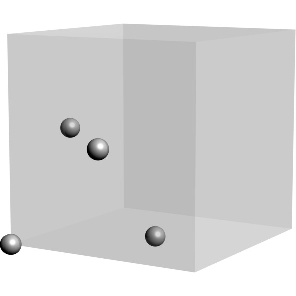
\includegraphics{fig.pdf}
\end{minipage}

where \(i\), \(j\) and \(k\) run from \(0\) to \(n-1\) and \(d\) is the size of one unit cell. One atom is placed at the bottom left corner of the unit cell, and the other three at
the centre of the three connected walls (see drawing above). This structure will contain \(4n^3\) atoms in total, and the total size of the simulation box will be $(nd)^3=L^3$.


\begin{enumerate}[label=\roman*.]
    \item Write a function which takes \(n\) and \(L\) (or \(n\) and \(d\)) as arguments and returns the positions of \(4n^3\) atoms on a face-centred cubic lattice.
    \item Verify your implementation by calling your function for \(n=3\) and \(L = 20\), writing the resulting positions to an \texttt{xyz}-file and looking at the result in Ovito. Your system should contain \(4\cdot3^3=108\) atoms.
    \item Show that the unit cell size corresponding to the density \(\rho=\SI{1.374}{\gram\per\cm\tothe3}\) is \(d=1.7 \sigma\). This will be used in the remaining parts of the project.
\end{enumerate}

\subsection{Many atoms, open boundary}
\begin{enumerate}[label=\roman*.]
    \item Simulate \(256\) atoms starting from rest, and visualise the results.
    \item Plot the potential, kinetic and total energy as a function of time. What is the main difference from the energy graphs for two and four atoms?
\end{enumerate}

\subsection{Boundary conditions}
In the previous exercise, you probably observed that the atoms immediately spread out into a large volume, possibly with some continuing to infinity (and beyond). This is not the behaviour we want. Ideally, we would like to model the bulk behaviour of argon by the use of periodic boundary conditions, but it is finicky to implement this efficiently.

Instead, we will model atoms which are forced to remain inside a box by the use of reflective boundary conditions. This gives reasonable results for the quantities that we want to measure.
Having reflective boundary conditions simply means that atoms that would otherwise leave the box, are turned around.
\begin{enumerate}[label=\roman*.]
    \item Implement reflective boundary conditions in your program.
    \item Run a simulation with \(108\) atoms and verify visually that your implementation works. Give the atoms some initial velocities of your own choosing.
\end{enumerate}


%           _
%  ___  ___(_) ___ _ __   ___ ___
% / __|/ __| |/ _ \ '_ \ / __/ _ \
% \__ \ (__| |  __/ | | | (_|  __/
% |___/\___|_|\___|_| |_|\___\___|
\section{\underline{Science}}
By now, you will have a well-functioning (if not terribly efficient) set of tools for running molecular dynamics simulations. It is now time to apply these tools to real problems. The goal is to reproduce some of the main results from the first article containing proper molecular dynamics (``landmark simulations'' according to Wikipedia\footnote{\url{https://en.wikipedia.org/wiki/Molecular_dynamics\#History}}), written by A. Rahman in 1964\cite{Rahman_1964}.

\subsection{Temperature}
\paragraph{Measurement:} Temperature is one of the most important concepts in thermodynamics, and you will learn much more about it in FYS2160. As you may have learnt already, temperature measures the vibrations of atoms. This is formalised through the equipartition theorem, which for a monoatomic gas such as argon states that
\[
    \ev{K} = \tfrac{3}{2}k_\mathrm{B}T,
\]
where \(\ev{K}\) is the average kinetic energy, \(T\) is the temperature and \(k_\mathrm{B}\) is Boltzmann's constant. In a molecular dynamics simulation, the temperature can be calculated by using the equipartition theorem ``backwards'', i.e.
\[
    T = \frac{2\ev{K}}{3k_\mathrm{B}} = \frac{\ev{mv^2}}{3k_\mathrm{B}} = \frac{m}{3k_\mathrm{B}N}\sum_i v_i^2.
\]
The sum runs over all atoms.

\paragraph{Units:} Note that since we are using reduced coordinates such as \(\vec{r}\,'=\vec{r}/\sigma\) and \(t'=t/\tau\), a direct calculation from the equation above gives a reduced temperature \(T'=T/T_0\), where \(T_0 = \varepsilon/k_\mathrm{B}=\SI{119.7}{\kelvin}\). In reduced units, the temperature expression is simplified to
\[
    T' = \frac{1}{3N}\sum_i v_i'^2.
\]
\begin{enumerate}[label=\roman*.]
    \item Extend your implementation with the calculation of temperature.
\end{enumerate}

\paragraph{Initialisation of velocities:} Velocities in a gas are usually distributed according to a normal distribution, i.e.~a Gaussian function, as you can see in figure 1 of~\cite{Rahman_1964}. In order to initialise a system with a given temperature, each component of the velocity of each atom should be randomly chosen from a normal distribution with mean zero and standard deviation \(\sqrt{kT/m}\). The following \texttt{numpy} command achieves this in reduced units:
\begin{lstlisting}
v0 = np.random.normal(0, sqrt(T), size=(N,3))
\end{lstlisting}

\begin{enumerate}[label=\roman*.,resume]
    \item Run a simulation with \(108\) atoms and an initial temperature of \(\SI{300}{\kelvin}\). Plot the temperature as a function of time.
\end{enumerate}

%                   __
% __   ____ _  ___ / _|
% \ \ / / _` |/ __| |_
%  \ V / (_| | (__|  _|
%   \_/ \__,_|\___|_|
\subsection{Velocity autocorrelation and diffusion coefficient}
The velocity autocorrelation, denoted \(A(t)\), is a measure of how similar the distribution of velocities is to the initial distribution. It is shown in figure 4 of~\cite{Rahman_1964}. \(A(t=0)=1\), since the velocity distribution at \(t=0\) \emph{is} the initial distribution, while \(A(t)\) decreases rapidly for \(t>0\) as the atoms collide with each other and the velocities become less and less similar to the initial distribution.

Mathematically, the velocity autocorrelation is defined as
\begin{equation}
    A(t) = \ev{\frac{\vec{v}(t)\cdot\vec{v}(0)}{\vec{v}(0)\cdot\vec{v}(0)}}
         = \frac{1}{N} \sum_i \frac{\vec{v}_i(t)\cdot\vec{v}_i(0)}{\vec{v}_i(0)\cdot\vec{v}_i(0)},\label{eq:vacf}
\end{equation}
where the sum runs over all atoms.

\begin{enumerate}[label=\roman*.]
    \item Add the calculation of the velocity autocorrelation to your implementation.
    \item Run a simulation with e.g. \(256\) atoms (more if you can), and plot the velocity autocorrelation as a function of time. Compare with figure 4 of~\cite{Rahman_1964}.
    \item Plot the temperature as a function of time, and find an initial temperature that makes the equilibrium temperature approximately equal to the \(\SI{94.4}{\kelvin}\) used in~\cite{Rahman_1964}.
\end{enumerate}

One cause of deviations is that the initial configuration of positions and velocities (\(\vec{v}_i(0)\) in~\vref{eq:vacf}) should be an equilibrium distribution.
\begin{enumerate}[label=\roman*.,resume]
    \item Use the final positions and velocities from the previous simulation as initial positions and velocities for a new simulation, and calculate and plot the new velocity autocorrelation.
    \item If your plot is very noisy (and your program does not run for too long), redo the two above simulations multiple times and average the velocity autocorrelation.
\end{enumerate}

The article also contains calculations of the diffusion coefficient \(D\), as shown in figure 3. Here, it is calculated as the slope of the mean squared displacement as a function of time. This requires periodic boundary conditions, which we have chosen to omit from this project. Fortunately, the diffusion coefficient can also be obtained from the velocity autocorrelation, via the Green-Kubo relation,
\[
    D = \frac{1}{3}\int_0^\infty A(t)\dd{t}.
\]
While it is not possible to integrate to \(\infty\) in a molecular dynamics simulation, the rapid decrease of \(\abs{A(t)}\) ensures that a finite integral will give a good approximation. Use your previous plot of \(A(t)\) to determine a reasonable upper bound.

\begin{enumerate}[label=\roman*.,resume]
    \item Estimate the diffusion coefficient from your previously calculated velocity autocorrelation. Compare with the result from~\cite{Rahman_1964}.
\end{enumerate}

%          _  __
%  _ __ __| |/ _|
% | '__/ _` | |_
% | | | (_| |  _|
% |_|  \__,_|_|
\subsection{Radial distribution function}
The radial distribution function \(g(r)\) shown in figure 2 of~\cite{Rahman_1964} describes the distribution of distances between an atom and its neighbours. It is defined as the ratio of the density at a distance \(r\) from an atom and the average density, i.e.
\begin{equation}
    g(r) = \frac{V}{N} \frac{n(r)}{4\pi r^2\Delta r},\label{eq:rdf}
\end{equation}
where \(V\) is the total volume, \(N\) the total number of particles and \(n(r)\) the average number of particles at a distance between \(r\) and \(r+\Delta r\). \(g(r)\) should be calculated for all atoms and then averaged. An example implementation is given below. The output should be averaged over many timesteps for a smooth result. Note that while \(g(r)\) should approach \(1\) when \(r\to\infty\) in bulk, the finite system size causes \(g(r)\) to decay for large \(r\).
\begin{enumerate}[label=\roman*.]
    \item Run  a simulation with as many atoms for as long as you can. Calculate the radial distribution function \(g(r)\), plot the result and compare with figure 2 of~\cite{Rahman_1964}.
\end{enumerate}
\lstinputlisting[linerange={rdfstart-rdfend}]{rdf.py}








\clearpage
\appendix
\section*{Appendix}
\setcounter{subsection}{0}
\addcontentsline{toc}{section}{Appendix}
\renewcommand{\thesubsection}{\Alph{subsection}}
\labelformat{subsection}{appendix~#1}

% __  ___   _ ____
% \ \/ / | | |_  /
%  >  <| |_| |/ /
% /_/\_\\__, /___|
%       |___/
\subsection{Data file format}\label{app:xyz}
The \texttt{xyz}-format is a semi-standard format for storing data from molecular dynamics simulations. Each time step is stored in the following format, and there are no blank lines between timesteps:
\begin{itemize}
    \item A line containing the number of atoms (an integer).
    \item An ignored line (this line is usually written as a header for the subsequent columns).
    \item One line for each atom, containing the atom type and the \(x\)-, \(y\)- and \(z\)-coordinates.
\end{itemize}
For two atoms simulated over three timesteps, where \texttt{xij} represents the \(x\)-coordinate of atom \(j\) at timestep \(i\), the file would look like this:
\begin{lstlisting}[language=]
    2
    type  x   y   z     <--- This line is a read as a comment, and therefore ignored.
    Ar   x11 y11 z11
    Ar   x12 y12 z12
    2
    type  x   y   z
    Ar   x21 y21 z21
    Ar   x22 y22 z22
    2
    type  x   y   z
    Ar   x31 y31 z31
    Ar   x32 y32 z32
\end{lstlisting}


%             _ _
%   _____   _(_) |_ ___
%  / _ \ \ / / | __/ _ \
% | (_) \ V /| | || (_) |
%  \___/ \_/ |_|\__\___/
\tikzexternaldisable
\subsection{Visualisation}\label{app:ovito}
Files written in the \texttt{xyz}-format can be read using the Ovito visualisation tool. It can be downloaded and installed from \url{https://ovito.org/index.php/download}.

When the installation has finished, simply open Ovito, click ``File'' \(\to\) ``Load File`` and choose your \texttt{xyz}-file. Edit the column mapping in the dialogue if necessary. When the atoms have appeared on your screen, check the box named ``File contains time series'' on the right-hand side, press \tikz[x=8pt,y=8pt]{\filldraw[fill=white] (0,0) -- (0,1) -- (0.866,0.5) -- (0,0);} and watch your atoms move around!

%                 _      _
% __   _____ _ __| | ___| |_
% \ \ / / _ \ '__| |/ _ \ __|
%  \ V /  __/ |  | |  __/ |_
%   \_/ \___|_|  |_|\___|\__|
\subsection{Velocity-Verlet}\label{app:verlet}
The Velocity-Verlet integration scheme is based on a second-order Taylor polynomial. With \(\vec{r}_i(t)\) denoting the position of atom \(i\) at a time \(t\), the second-order Taylor expansions of position and velocity can be written as
\begin{alignat*}{2}
    \vec{r}_i(t+\Delta t) &\approx \vec{r}_i(t) + \vec{v}_i(t)\Delta t + \tfrac{1}{2}\vec{a}_i(t)\Delta t^2\\
    \vec{v}_i(t+\Delta t) &\approx \vec{v}_i(t) + \vec{a}_i(t)\Delta t + \tfrac{1}{2}\vec{a}_i'(t)\Delta t^2.
\end{alignat*}
There is no explicit expression for \(\vec{a}'(t)\). It can, however, be approximated using our old friend
\[
\vec{a}\,'(t)\approx\frac{\vec{a}(t+\Delta t)-\vec{a}(t)}{\Delta t}.
\]
Since the acceleration is independent of the velocity, the newly updated position, \(\vec{r}(t+\Delta t)\), is sufficient to calculate \(\vec{a}(t+h)\). Inserting this into the expression for \(\vec{v}(t+\Delta t)\), we get
\begin{alignat*}{2}
    \vec{v}_i(t+\Delta t) &\approx \vec{v}_i(t) + \vec{a}_i(t)\Delta t + \tfrac{1}{2}\qty(\vec{a}_i(t+\Delta t)-\vec{a}_i(t))\Delta t\\
    &= \vec{v}_i(t) + \tfrac{1}{2}\qty(\vec{a}_i(t)+\vec{a}_i(t+\Delta t))\Delta t.
\end{alignat*}
The discretised algorithm then becomes
\begin{alignat*}{2}
    \vec{r}_{i,j+1} &\approx \vec{r}_{i,j} + \vec{v}_{i,j}\Delta t + \tfrac{1}{2}\vec{a}_{i,j}\Delta t^2\\
    \vec{v}_{i,j+1} &\approx \vec{v}_{i,j} + \tfrac{1}{2}\qty(\vec{a}_{i,j} + \vec{a}_{i,j+1})\Delta t,
\end{alignat*}
where \(\vec{r}_{i,j}\) is the position of atom \(i\) at timestep \(j\). In your implementation, you should avoid having to calculate the acceleration more than once per timestep.



\nocite{*}
\printbibliography{}
\addcontentsline{toc}{chapter}{\bibname}
\end{document}
